\section{DevOps}
DevOps ist eine Organisationsform, mit der Continuous Delivery optimal funktioniert. Im Zentrum steht das Zusammenspiel von Entwicklung (Developement) und Betrieb (Operations), wodurch bereits das Wesentliche des Gedankens hervorgeht: Ein Zusammenwachsen der beiden Abteilungen zu einem Verband. Dabei fokussiert sich dieser Ansatz auf die Liefergeschwindigkeit, das kontinuierliche Testen in produktionsähnlichen Umgebungen, kontinuierliche Rückmeldung und schnelle Reaktionsfähigkeit. Jedes Team ist somit für eine Domäne zuständig und kann diese unabhängig von anderen Teams als Service implementieren. Der Dienst kann schließlich selbständig optimiert werden, um einen guten Betrieb zu ermöglichen. Des Weiteren kann ohne weitere Abstimmung eine Weiterentwicklung am Dienst vorgenommen werden. Die Teams übernehmen die vollständige Verantwortung für ihre Komponenten und den eingesetzten Technologie-Stack. Daraus folgt eine geringe Koordination untereinander, wodurch wiederum Software schneller entwickelt und in Produktion gebracht werden kann \cite{Wolff.2016}. Das Zusammenspiel dieser Abteilungen ist in Abbildung \ref{fig:devops} dargestellt. Auch die Qualitätssicherung ist hier mit inbegriffen. \\ \\
In klassischen Organisationsformen sind Entwicklung und Betrieb in mindestens zwei unterschiedliche Abteilungen getrennt und verfolgen verschiedene Ziele. Während bei dem Betrieb Kosteneffizienz in den Vordergrund rückt, stellt die Entwicklung neue Features bereit und wird anhand der Geschwindigkeit und Effizienz ihres Vorgehens gemessen. Wird Continuous Delivery eingeführt, sollten Betrieb und Entwicklung Hand in Hand arbeiten, um das Notwendige Wissen und entsprechende Werkzeuge zu teilen. Jede Abteilung beherrscht durch die unterschiedliche Perspektive auf die Anwendungen einen Teil von Continuous Delivery. Ohne Monitoring, Security oder Netzinfrastrukturen kann eine Anwendung nicht sinnvoll realisiert oder betrieben werden. Der Betrieb ist für diese Aspekte zuständig, wohingegen die Entwicklung den Code, die Entwicklungsinfrastruktur und Middleware wie Application Server kennt. Gemeinsam lässt sich somit eine Continuous-Delivery-Pipeline aufbauen. Mit der Einführung von Continuous Delivery sollte allerdings auch die Einführung von DevOps in Betracht gezogen werden \cite{Wolff.2016}.\\ \\
Continuous Delivery wird häufig mit DevOps gleichgesetzt. Das trifft jedoch nicht zu. Durch DevOps lässt sich Continuous Delivery zwar vereinfachen, allerdings gibt es neben dieser (wesentlichen) Praktik im DevOps-Umfeld noch weitere Bereiche (Monitoring, Troubleshooting), bei denen diese Organisationsform und eine damit einhergehende Zusammenarbeit sinnvoll sein kann \cite{Wolff.2016}.
\begin{figure*}[h!]
	\centering
	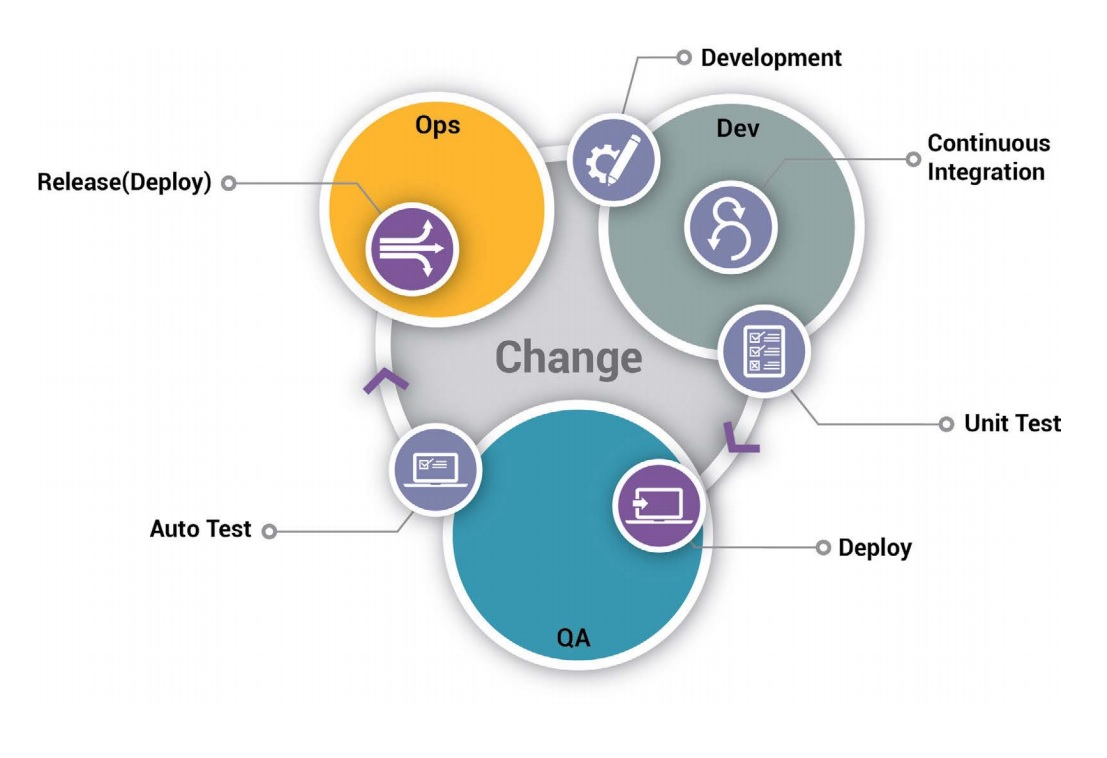
\includegraphics[width=0.8\linewidth]{images/devops2}
	\caption{Wandel von klassischer Organisation zu DevOps-Teams} 
	%https://www.microfocus.com/media/ebook/Software-DevOps-eBook.pdf
	\label{fig:devops}
\end{figure*}
